% Standalone main paper, including references. Compile supplyment.tex separately.
\documentclass[10pt,twocolumn,letterpaper]{article}
\usepackage[review]{cvpr}
\usepackage[T1]{fontenc}
\usepackage{amsmath,amssymb,graphicx,booktabs,multirow,tabularx,microtype,xspace}
\usepackage{dblfloatfix}
\newcommand{\method}{REVEAL\xspace}
\newcommand{\R}{\mathbb{R}}
\newcommand{\TODO}[1]{\textbf{\textcolor{red!70!black}{[TODO: #1]}}}
\newcommand{\pending}{\textcolor{red!70!black}{TODO}}
\DeclareMathOperator{\clip}{clip}
\DeclareMathOperator{\sigmoid}{sigmoid}
\DeclareMathOperator{\logit}{logit}
\DeclareMathOperator*{\argmin}{arg\,min}

\newcommand{\MainResultRows}{%
Rule VLM (bare) & 13/39 & 33.3 & [20.6, 49.0] & 14/40 & 15 \\
Fine-tuned VLM (bare) & 26/39 & 66.7 & [51.0, 79.4] & 27/40 & 9 \\
AIMI & 29/39 & 74.4 & [58.9, 85.4] & 29/40 & 10 \\
}
\newcommand{\AblationResultRows}{%
Fixed 0.15 & Student & 23/40 & 16 & 20/37 & 54.1 \\
Learned & Student & 26/40 & 11 & 25/37 & 67.6 \\
Fixed 0.15 & Learned & 28/40 & 8 & 26/37 & 70.3 \\
Learned & Learned & 29/40 & 10 & 27/37 & 73.0 \\
}
\newcommand{\StudentResultRows}{%
Released pose-goal student & 39/40 & 1 \\
Frozen latent student & 38/40 & 2 \\
Latent + simulated-noise DAgger & 39/40 & 1 \\
Latent + CNN-feedback DAgger & 40/40 & 0 \\
}

\newcommand{\QOneOriginalSuccess}{70.4}
\newcommand{\QOneChangedSuccess}{65.8}
\newcommand{\QOneOriginalGain}{26.2}
\newcommand{\QOneChangedGain}{40.4}
\newcommand{\QOneOriginalBaseline}{44.2}
\newcommand{\QOneChangedBaseline}{25.4}
\newcommand{\QOneAverageRow}{%
Mean & -- & 43.0 & 44.2 & 40.4 & \textbf{70.4} & 25.4 & 10.0 & 10.8 & \textbf{65.8}\\
}

\newcommand{\HardwareRuleSuccess}{40.0}
\newcommand{\HardwareFineTunedSuccess}{66.25}
\newcommand{\HardwareFineTunedCtrlSuccess}{62.5}
\newcommand{\HardwareAimiSuccess}{87.5}
\newcommand{\HardwareGain}{21.25}
\newcommand{\HardwareCtrlGain}{25.0}
\newcommand{\HardwareCtrlDelta}{3.75}

\newcommand{\FollowupPhaseRows}{%
Fixed & Student & 20/37 & 4 & 0 & 12 \\
Learned & Student & 25/37 & 1 & 3 & 6 \\
Fixed & Learned & 26/37 & 4 & 0 & 4 \\
Learned & Learned & 27/37 & 0 & 1 & 9 \\
}
\newcommand{\FollowupReplicationRows}{%
REVEAL & 26/37 & 70.3 \\
Fine-tuned VLM, bare & 27/37 & 73.0 \\
Rule VLM, bare & 21/37 & 56.8 \\
}
\newcommand{\FollowupPairRows}{%
Explicit actor goal & 26/38 & 5 \\
No explicit actor goal & 29/38 & 2 \\
}
\newcommand{\FollowupVisualRows}{%
Fine-tuned VLM & 30/40 & 16/40 & 3/40 \\
Rule VLM & 23/40 & 23/40 & 0/40 \\
}
\newcommand{\FollowupVisualBindingRows}{%
Fine-tuned & Identity & 34 & 4 & 2 & -- \\
Fine-tuned & Permuted & 25 & 11 & 4 & 9 \\
Fine-tuned & Masked & 3 & 1 & 36 & -- \\
Rule & Identity & 24 & 6 & 10 & -- \\
Rule & Permuted & 25 & 6 & 9 & 3 \\
Rule & Masked & 0 & 0 & 40 & -- \\
}

\newcommand{\CompletedNativeRows}{%
REVEAL & 35/40 & 87.5 & [73.9, 94.5] & 3 & 101 \\
Fine-tuned VLM, bare & 30/40 & 75.0 & [59.8, 85.8] & 9 & 117 \\
Rule VLM, bare & 17/40 & 42.5 & [28.5, 57.8] & 12 & 126 \\
}
\newcommand{\CompletedWaitingRows}{%
Original waiting & 27/39 & 69.2 & 10 & 28/40 \\
Refitted waiting & 33/39 & 84.6 & 5 & 33/40 \\
}
\newcommand{\CompletedFeedbackRows}{%
One initial plan & 7/39 & 17.9 & 40 \\
Full feedback & 30/39 & 76.9 & 113 \\
}
\newcommand{\CompletedGoalRows}{%
Correct goal & 25/36 & 69.4 \\
No explicit goal & 24/36 & 66.7 \\
Shuffled goal & 30/36 & 83.3 \\
}
\newcommand{\CompletedVisualRows}{%
REVEAL & 32/40 & 32/40 & 0/39 \\
Fine-tuned VLM, bare & 30/40 & 16/40 & 3/40 \\
Rule VLM, bare & 23/40 & 23/40 & 0/40 \\
}
\newcommand{\CompletedCloudRows}{%
Original execution & 29/40 & 3 \\
Fixed residual gate & 27/40 & 7 \\
Phase-fixed gate & 24/40 & 10 \\
Learned residual gate & 26/40 & 5 \\
}

\newcommand{\AblationWaitingRows}{%
Continue student & 25/40 & 62.5 & 12 & 7\\
Fixed slowdown & 30/40 & 75.0 & 4 & 4\\
Learned slowdown & 28/40 & 70.0 & 8 & 1\\
Learned slowdown + correction & 34/40 & 85.0 & 5 & 4\\
}
\newcommand{\AblationFeedbackRows}{%
One initial plan & 6/39 & 15.4 & 0 & 40\\
Full feedback & 33/39 & 84.6 & 5 & 120\\
}
\newcommand{\AblationRawRows}{%
Continue student & 25 & 12 & 2 & 1 & 0 & 0 & 104\\
Fixed slowdown & 30 & 4 & 2 & 3 & 1 & 0 & 132\\
Learned slowdown & 28 & 8 & 2 & 2 & 0 & 0 & 113\\
Learned slowdown + correction & 34 & 5 & 1 & 0 & 0 & 0 & 120\\
One initial plan & 6 & 0 & 5 & 28 & 0 & 1 & 40\\
}
\newcommand{\AblationPhaseRows}{%
Continue student & 4 & 3 & 5 & 12\\
Fixed slowdown & 4 & 0 & 0 & 4\\
Learned slowdown & 0 & 1 & 7 & 8\\
Learned slowdown + correction & 0 & 4 & 1 & 5\\
}

\newcommand{\ImageRefreshRows}{%
Current image & 32/40 & 80.0 & 3 & 112\\
Repeated first frame & 9/40 & 22.5 & 4 & 98\\
}

% Generated by scripts/render_q3_inspection.py; distinct Q3(c) cohort.
\newcommand{\InspectionPolicyRows}{%
Fixed sweep & 31/40 & 77.5 & 1 & 126\\
Adaptive inspection & 38/40 & 95.0 & 0 & 117\\
}

% Generated by scripts/render_q3_pig_inspection.py from the 80 raw formal records.
\newcommand{\PigInspectionPolicyRows}{%
Fixed sweep & 29/40 & 72.5 & 2 & 125\\
Adaptive inspection & 37/40 & 92.5 & 2 & 106\\
}

\newcommand{\DiceLayoutRows}{%
AIMI & 28/40 & 26/40\\
Fine-tuned VLM, bare & 23/40 & 0/40\\
Rule VLM, bare & 13/40 & 1/40\\
}
\newcommand{\DiceLayoutTestRows}{%
I: AIMI vs. fine-tuned & 11 & 6 & 0.3323\\
I: AIMI vs. rule & 18 & 3 & 0.0015\\
P: AIMI vs. fine-tuned & 26 & 0 & $2.98\times10^{-8}$\\
P: AIMI vs. rule & 25 & 0 & $5.96\times10^{-8}$\\
AIMI: I vs. P & 4 & 2 & 0.6875\\
Fine-tuned: I vs. P & 23 & 0 & $2.38\times10^{-7}$\\
Rule: I vs. P & 13 & 1 & 0.0018\\
}

\definecolor{cvprblue}{rgb}{0.21,0.49,0.74}
\usepackage[pagebackref,breaklinks,colorlinks,allcolors=cvprblue]{hyperref}
\def\confName{CVPR}\def\confYear{2027}
\title{REVEAL: Agentic In-Hand Manipulation for Language-Guided Visual Exploration}
\hypersetup{pdftitle={REVEAL: Agentic In-Hand Manipulation for Language-Guided Visual Exploration},pdfauthor={Anonymous submission}}
\author{Anonymous submission}
% Compact the anonymous-author block for the enlarged teaser (local override).
% The CVPR style file, text size, page margins and abstract remain unchanged.
\makeatletter
\patchcmd{\@maketitle}{\vspace*{24pt}}{\vspace*{4pt}}{}{\PackageError{reveal-layout}{Title spacing patch failed}{}}
\patchcmd{\@maketitle}{\vskip .5em}{\vskip 0pt}{}{\PackageError{reveal-layout}{Author spacing patch failed}{}}
\patchcmd{\@maketitle}{\vspace*{12pt}}{\vspace*{2pt}}{}{\PackageError{reveal-layout}{Title footer spacing patch failed}{}}
\makeatother
\begin{document}
\raggedbottom
% Restore standard float spacing and give table rows a little more room.
\AtBeginEnvironment{table}{\renewcommand{\arraystretch}{1.10}}
\twocolumn[{
\maketitle
\vspace{-12pt}
\begingroup
\centering
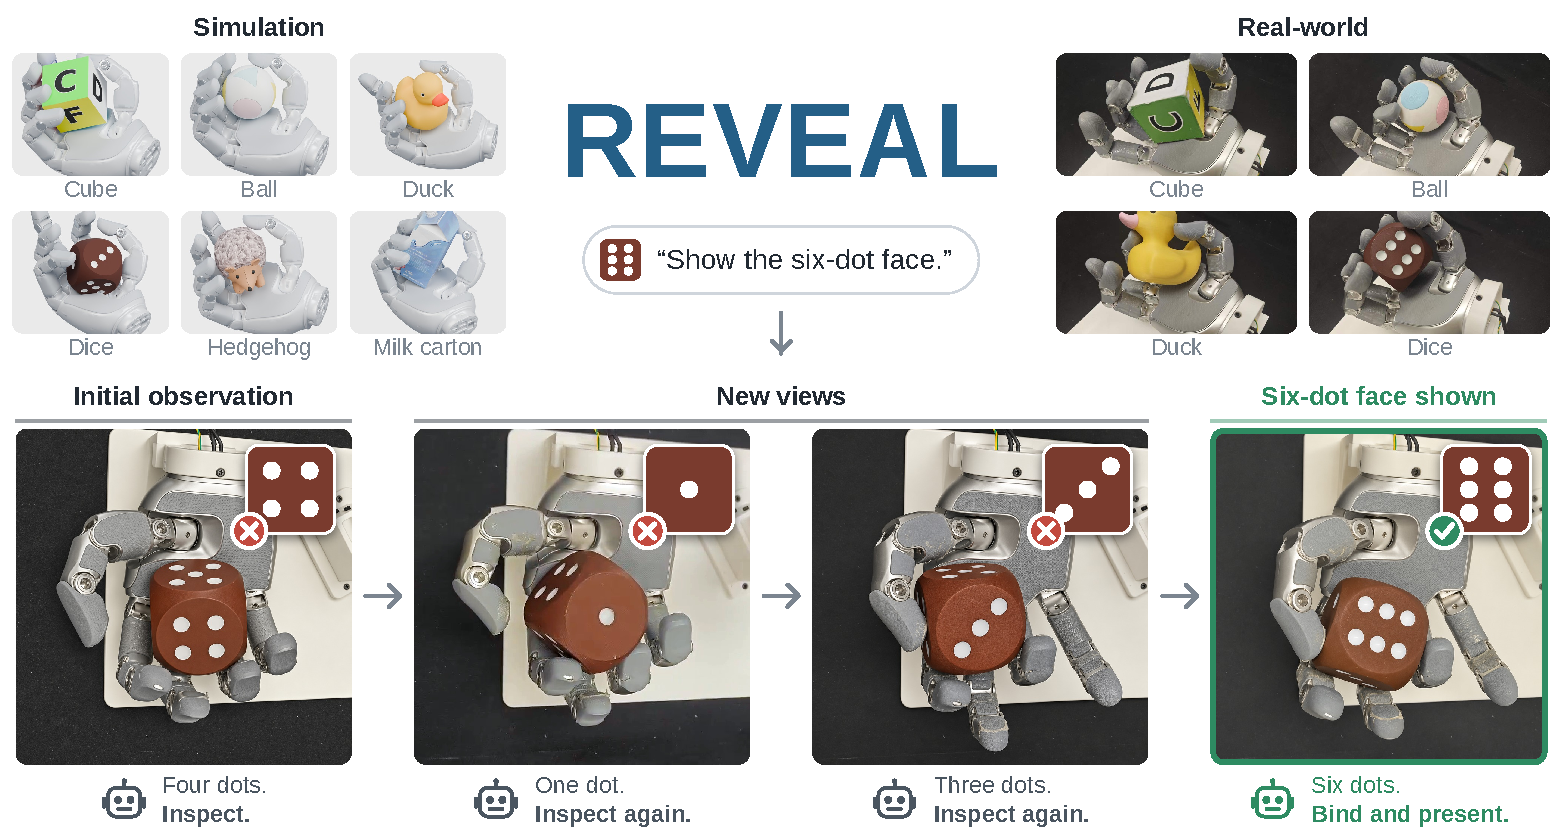
\includegraphics[width=0.98\textwidth]{figures/imported/v24/reveal_teaser_v24.pdf}
\par
\captionof{figure}{\textbf{Language-guided visual exploration.} A language instruction guides inspection and presentation of the six-dot face. Top: simulated and physical objects. Bottom: real video frames with schematic face and agent-decision annotations.}
\label{fig:teaser}
\par\endgroup
\vspace{6pt}
}]
\begin{abstract}
A language-specified target may be hidden from the camera during in-hand manipulation, so the robot must gather visual evidence before it can present the target. We introduce REVEAL, an agentic framework that coordinates visual exploration with continuous hand control. The agent selects inspection directions and durations, uses new RGB observations and state feedback to bind the requested target to a motor goal, and guides its presentation. An occlusion-robust pose estimator and teacher-supervised local controllers keep the object tracked and stable during reasoning and execution. Controlled studies isolate the roles of fresh visual evidence, inspection choices, and control during reasoning. Across six object-specific simulation systems, our framework achieves \QOneChangedSuccess\% mean success under changed target-to-skill mappings, exceeding the strongest baseline by \QOneChangedGain{} percentage points. It transfers to four real-world objects, achieving \HardwareAimiSuccess\% success over 80 trials, compared with \HardwareFineTunedSuccess\% for the strongest baseline; giving that baseline the same local controllers does not close the gap, which locates the physical gain in exploration rather than in low-level control. On real images, our pose estimator reaches 87.3\% recall against 40.7\% for a keypoint baseline.
\end{abstract}

% Two-column system overview, queued early so it lands before the method text.
\begin{figure*}[!t]
\centering
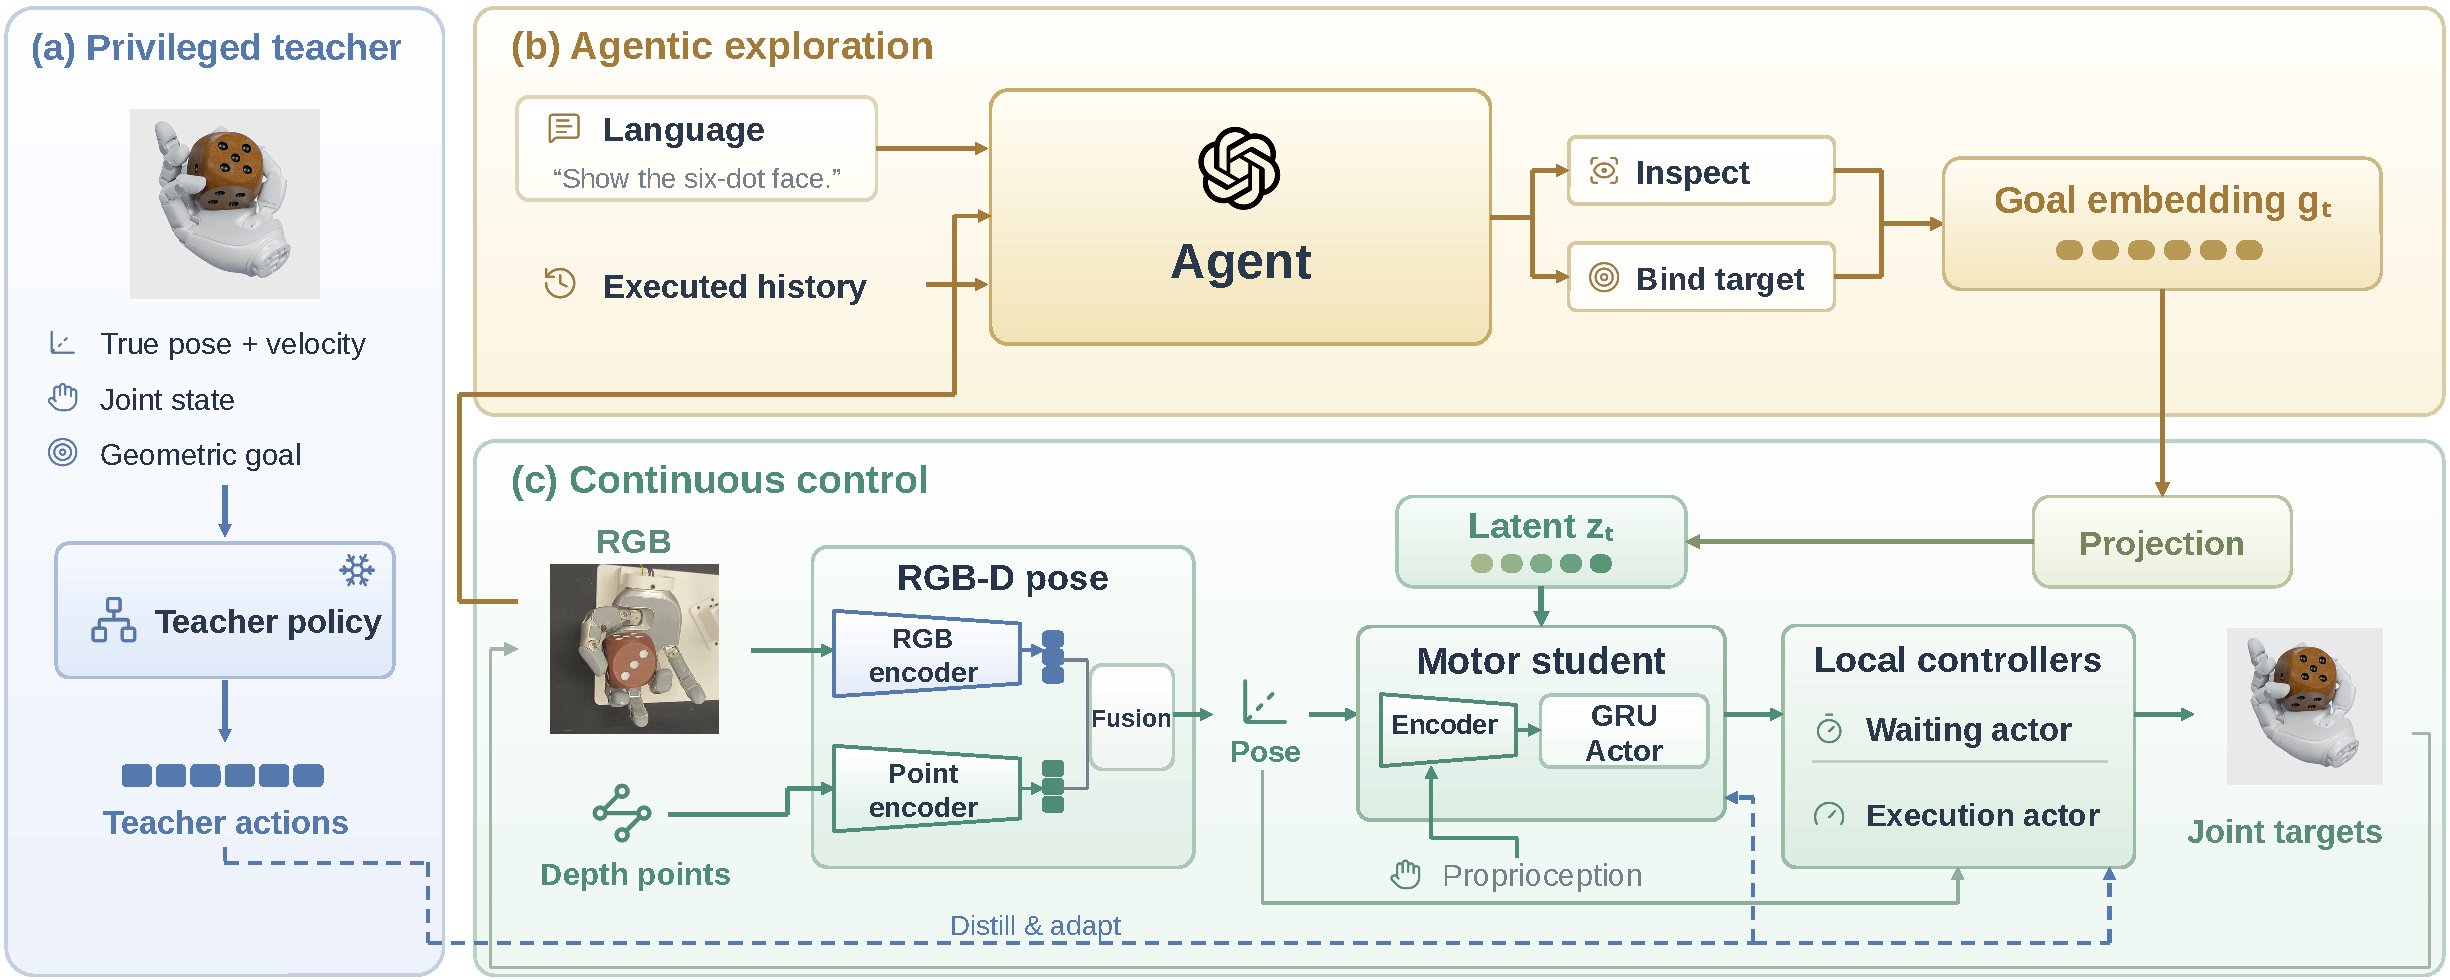
\includegraphics[width=0.96\textwidth]{figures/imported/v11/reveal_pipeline_v11.pdf}
\caption{\textbf{REVEAL training and deployment.} (a) A privileged teacher with full simulator state is trained for the Revo3 hand. (b) At deployment the agent reads the instruction, the current view and the history of executed actions, and returns either an inspection or a target binding; its output is a goal embedding $g_t$ drawn from the skill bank. (c) Underneath, an RGB-D pose estimator fuses image features with measured surface points, a motor student turns pose and goal into joint targets, and waiting and execution controllers adjust those targets while the agent is still reasoning. The teacher is used only for supervision and the state decoder only in training.}
\label{fig:pipeline}
\end{figure*}

\section{Introduction}
A robot hand that holds an object also hides it. Fingers cover part of the surface, and whatever faces the palm or points away from the camera cannot be seen at all. For most learned in-hand controllers this is a nuisance for state estimation and nothing more, because the goal is given in advance as a target pose or a goal image~\cite{bhardwaj2026viserdex,bhardwaj2026goaldex,kedia2026simtoolreal}. It becomes the central problem once the goal is given in language. Asked to ``present the face marked T,'' the robot may be looking at a cube whose T is on the far side, and nothing in the current image tells it which orientation the instruction refers to (Fig.~\ref{fig:teaser}).

The robot has to look before it can act: turn the object, take another view, read the mark, and only then commit to an orientation. This is active perception~\cite{bajcsy1988active,bohg2017interactive}, except that the viewpoint is moved by contact-rich finger motion and a poor choice can drop the object. A vision-language model can reason about which view to obtain next, but it takes seconds to answer (about five in our trials), and during those seconds the object still has to be tracked and held at every control step, under exactly the finger occlusion that inspection produces.

REVEAL treats this as two visual processes at different rates. A slow \emph{semantic} process decides what is on the object: an agent reads the instruction and the current image, chooses the direction and duration of each inspection, and, once a view shows the requested mark, links that surface to a motor goal. We call this \emph{target binding}, and it is what turns ``the face marked T'' into a skill the hand can execute. A fast \emph{geometric} process tracks where the object is: an RGB-D network fuses image features with measured surface points to estimate pose at every control step, and this pose drives a goal-conditioned policy for the Revo3 hand. Two teacher-supervised local controllers bridge the two rates, holding the object stable while a reply is pending and correcting the policy's commands once a goal is bound.

Controlled studies change one ingredient at a time, and each of these parts earns its place: fresh images, not repeated ones, account for the benefit of feedback; agent-chosen inspections beat a fixed sweep; learned slowing with joint correction beats both fixed slowing and uninterrupted execution. As a complete system, REVEAL reaches \QOneChangedSuccess\% mean success on six simulated objects under changed target-to-skill mappings, \QOneChangedGain{} points above the strongest baseline, and \HardwareAimiSuccess\% over 80 real-hand trials on four objects, where a baseline carrying the same local controllers reaches only \HardwareFineTunedCtrlSuccess\%. Our contributions are:
\begin{itemize}
\item An agentic framework for in-hand visual exploration, in which the agent chooses how to look and binds a visual target to a motor goal from successive observations.
\item A perception and control layer that holds the object steady while the agent reasons, combining an occlusion-robust RGB-D pose estimator with teacher-supervised local controllers.
\item Controlled studies isolating fresh observations, inspection choice and waiting control, with six-object, changed-mapping, two-language and four-object real-hand evaluations.
\end{itemize}

\section{Related Work}
\paragraph{Language-driven agents and active perception.}
Language-based agents connect task descriptions to robot actions by selecting skills~\cite{ichter2023saycan}, revising plans from feedback~\cite{huang2023innermonologue}, writing programs over perception and control APIs~\cite{liang2022codepolicies}, or expressing goals as spatial value maps and keypoint constraints~\cite{huang2023voxposer,huang2025rekep}; recent models connect multimodal and video backbones to actions more directly~\cite{yang2025magma,li2026vera}. At a broader level, ENPIRE casts agentic robotics as a closed loop that executes, verifies and refines policies on physical systems~\cite{xiao2026enpire}. These systems mostly reason about scenes whose relevant evidence is already visible. Moving a sensor or an object to obtain a more informative view is the subject of active and interactive perception~\cite{bajcsy1988active,bohg2017interactive}. We bring the two together inside a grasp: the agent has to produce the views it reasons about, each new view is a contact-rich reorientation, and what it resolves is a language-specified target.

\paragraph{Dexterous in-hand manipulation.}
Simulation-trained RL has brought in-hand reorientation and rotation to physical hands~\cite{openai2018dexterity,chen2022reorientation,qi2023hora}, with later work adding vision and touch~\cite{qi2023rotateit,yang2025anyrotate} and residual learning for transfer~\cite{li2025maniptrans}. Recent visual systems reach target poses from monocular RGB~\cite{bhardwaj2026viserdex}, follow goal images that a VLM can select from language~\cite{bhardwaj2026goaldex}, or share one goal-reaching policy across tools~\cite{kedia2026simtoolreal}. All of them start from a goal that can be specified up front. We address the step before it: finding out, through exploration, which goal the instruction refers to.

\paragraph{Control under inference delay.}
Large models answer more slowly than robots move. Real-time chunking~\cite{black2025rtc}, online action correction~\cite{sendai2025a2c2}, delay-aware preference learning~\cite{zhu2026deflect} and latency-aware RL~\cite{zhu2026arli} keep action-generating policies consistent across inference delays, and LiMA separates sparse intent generation from fast execution~\cite{chen2026lima}. In our setting the pending reply is a discrete goal and the delay lasts seconds, so the waiting controller learns to hold the object in the meantime, with no future action chunk to anticipate.

\section{Method}
\label{sec:method}
REVEAL answers two visual questions at two rates (Fig.~\ref{fig:pipeline}). \emph{What is on the object} is answered every few seconds by an agent that looks at RGB images and decides how to inspect. \emph{Where the object is} is answered at every control step by an RGB-D pose estimator, whose output drives a recurrent motor policy and two local controllers. Training has three stages: a privileged teacher and its distilled student for the Revo3 hand, adaptation of the student to a goal embedding produced by the agent, and learning of the local controllers. Every object goes through the same pipeline and has its own weights. We use the cube as the running example.

\subsection{Problem formulation}
\label{sec:task}
The robot holds an object and receives an instruction $\ell$ that names a surface target, such as a letter printed on one face. Each target has a \emph{presentation pose}: a fixed reference orientation of the object in which that target faces up. We call each of these six reference orientations a \emph{skill}, so that naming a target and naming a skill come to the same thing. The task is to bring the object to the presentation pose of the requested target and stop there, without dropping it. We score the full orientation, including rotation about the face normal, so that the mark is always shown the same way. This is stricter than merely exposing the correct face. Because the target may not be identifiable in the first image, hand motion serves two purposes: it exposes new views, and it later carries the object to the presentation pose.

At step $t$ the agent receives an RGB image $I_t$, the instruction, the history of executed actions and a summary of measured state, and emits a goal embedding $g_t$, a vector that names the skill to execute. The motor policy takes proprioception and history $x_t$, the measured object pose $\hat p_t$ and its recurrent state $h_t$, and proposes joint targets $u_t$. Local controllers turn these proposals into commands $a_t$. We write $m_t=1$ while an agent request is pending. Inspecting and binding are separate decisions: an inspection skill turns the object to obtain a view, and the target is bound only when the agent says so.


\subsection{Goal-Conditioned Motor Skills}
\paragraph{Teacher--student foundation.}
We train a teacher and a student for the Revo3 hand following ViserDex~\cite{bhardwaj2026viserdex}. The teacher uses privileged simulation state and geometric goals. It stays frozen and supplies the action labels for everything that follows. The student keeps its encoders, recurrent core and actor.

\paragraph{Goal-embedding adaptation.}
The original student is told where to go by a target quaternion. An agent cannot supply one before it has seen the target, so we give the student a discrete interface instead. A goal embedding $g_t$ is a 768-dimensional vector drawn from a bank $B=\{g_1,\ldots,g_6\}$ of six, one per skill, each corresponding to a reference object orientation. The vectors are precomputed text embeddings of the skill names~\cite{tschannen2025siglip2}. A learned projection replaces the student's geometric goal inputs:
\begin{align}
 z_t&=\tanh(W_g g_t+b_g),\\
 (u_t,h_{t+1})&=\pi_\theta([x_t,z_t],\hat p_t,h_t).
\label{eq:student}
\end{align}
The adapted student receives neither the target quaternion nor the relative-goal quaternion. The embedding the agent emits is resolved against $B$, so a command names a skill rather than a pose, and the student never sees an orientation it cannot be told.

We fit the projection and the recurrent policy to the frozen teacher's actions with a DAgger-style procedure~\cite{ross2011dagger}. The projection is first warmed up with an action MSE loss. Recurrent adaptation then adds a decoder that reconstructs the normalized privileged state, with the goal quaternion removed, under an MSE loss of weight 0.2. The teacher and the decoder are used only in training. Network dimensions and fitting details are in the supplement.

\subsection{Semantic Vision: Exploration and Target Binding}
\label{sec:exploration}
\begin{figure}[!b]
\centering
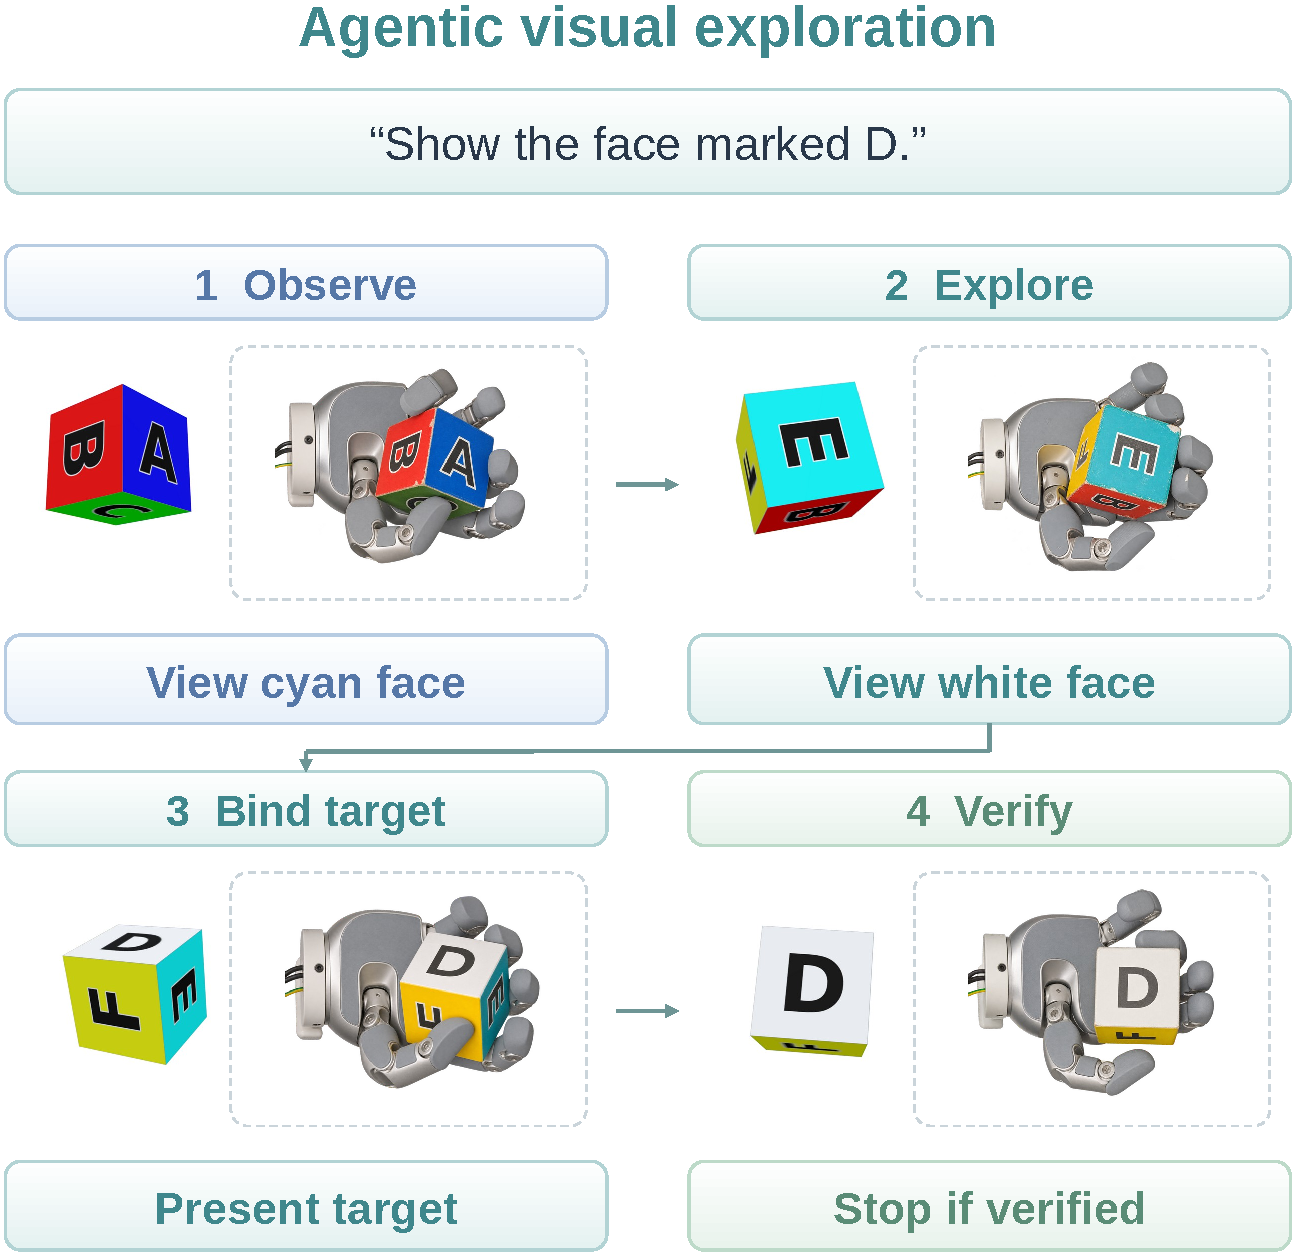
\includegraphics[width=\columnwidth]{figures/imported/v11/reveal_exploration_v11.pdf}
\caption{\textbf{Agentic visual exploration.} Given a request whose face is not in view, the agent observes, chooses an inspection that exposes new faces, binds the target once it appears, and stops only after the requested face is presented. Every step is a decision from the image and the action history, not a fixed schedule.}
\label{fig:exploration}
\end{figure}

At each call the agent receives the instruction, the current image, the history of executed actions and a summary of measured state, and returns one action: inspect, reorient, bind, verify, stop, or abstain. The image is the camera view of the hand and the object, so the requested mark may be turned away, covered by a finger or seen at a grazing angle. The state summary contains estimated skill-relative errors and the current binding and request status. It contains neither the true pose nor any correctness label. \emph{Inspection} selects a skill in order to obtain another view. \emph{Reorient} turns the object toward a face the agent wants to look at without claiming to have identified the target. \emph{Verify} asks for one more view before committing, \emph{stop} ends the trial once the agent believes the presentation is complete, and \emph{abstain} ends it as a failure, which is what the agent does when it cannot see the target. Replies are validated before they are applied, and an invalid reply leaves the current skill unchanged.

\paragraph{What a binding is.}
Target binding is the one action that turns a visual observation into a motor command, so it is worth defining exactly. The agent has a fixed dictionary of six skills, one per coloured face, and this dictionary is shared by every system and never learned. What the agent must supply is the second half: which skill ID corresponds to the requested mark. A binding is the agent's declaration of that pair, written as a skill ID $k$ together with the requested mark $m$, and it is applied only if $k$ is one of the six IDs and $m$ is the mark named in the instruction. Once applied, the skill ID becomes the active goal embedding $g_t$ and the object is driven toward that skill's presentation pose.

A binding is therefore reproducible without reference to the agent's reasoning. From a recorded trial one can read the declared pair, the skill that was actually executed, and whether the pair matches the instruction's mark under the trial's mapping. We call a binding \emph{correct} when the applied skill brings the requested mark to its presentation pose, which is checkable from the mapping and the skill dictionary alone. Reassignment, chosen inspections and retries can all change which pair is declared, but they do not change what the pair means, so the same definition scores every system in every experiment.

The agent also chooses how long each inspection or reorientation lasts, between 10 and 90 control steps. A short action gives a quick glimpse. A long one carries the object further toward the selected orientation. The next image shows the effect of the action and informs the next decision. Only one request can be pending at a time, and the current skill stays active until a valid reply changes it. The hand can therefore keep gathering evidence until the agent is ready to commit to a presentation goal.

\subsection{Geometric Vision: Pose Under Hand Occlusion}
\label{sec:pose}
The motor policy needs the object pose at every control step, and inspection is when pose is hardest to see: fingers cross in front of the object and large parts of it leave the view. A network that sees only RGB must then infer metric depth from appearance. We instead fuse the image with measured depth. The inputs are the segmented RGB image and up to 1,024 measured surface points of the object, each paired with its pixel location. A ResNet-34 encodes the image, and the feature at each point's pixel is sampled from the resulting map. A per-point MLP encodes the point's 3D position relative to the centroid of the observed points. The two features are concatenated, processed point-wise and max-pooled into a single vector, from which the network regresses the 3D positions of the object center and the eight corners of its bounding box in the camera frame. A rigid fit of the known keypoint layout to these predictions gives position, orientation and a fitting error, which is also passed to the local controllers. Depth anchors the estimate in metric space, while color resolves which face is which. The network is trained in simulation on Gaussian-splat renderings~\cite{bhardwaj2026viserdex} with hand occlusion, depth noise and point dropout, and the same design is used for all simulated objects and on the physical hand.

\subsection{Local Control During and After Reasoning}
\label{sec:wait}
The agent chooses goals at irregular intervals, but the hand needs a command at every control step. We place local controllers between the adapted student and the joints. A sensor encoder and a goal encoder feed a fusion layer that predicts corrections to the student's commands. The sensor features are proprioception, measured pose, the student's recurrent state and proposal, the pose-fitting error, and the binding and request status.

\paragraph{Waiting and execution commands.}
When a request is issued, we record the current pose and command as the \emph{request anchor}. The waiting actor receives this anchor and the elapsed waiting time, and predicts a speed logit $r_t$ and joint correction values $v_t$. With normalized current joints $\bar q_t$ and clipped student targets $\bar u_t$, the command is
\begin{align}
 \alpha_t&=\sigmoid(4r_t+\logit(0.15)),\\
 b_t&=\begin{cases}
 \bar q_t+\alpha_t(\bar u_t-\bar q_t),&m_t=1,\\
 \bar u_t,&m_t=0,
 \end{cases}\\
 a_t&=\clip\bigl(b_t+0.35\tanh(v_t),-1,1\bigr).
\label{eq:control}
\end{align}
While waiting, the hand moves toward the student's proposal at a learned fraction $\alpha_t$ of full speed. Zero actor outputs recover fixed slowing with coefficient 0.15. Slowing only scales the student's motion. The joint correction $v_t$ can also change its direction. When no request is pending, a separate execution actor supplies $v_t$ and the proposal is followed at full speed.

\paragraph{Teacher-supervised correction.}
The frozen teacher provides the labels for both actors: actions that hold the request anchor during waiting, and actions toward the active goal during execution. Each actor is trained against these labels with a penalty on its correction $\delta_\phi=0.35\tanh(v_t)$:
\begin{equation}
 \mathcal{L}_{\mathrm{control}}=\mathbb{E}_{(s,g,a^*)\sim\mathcal{D}}\left[\|a_\phi(s,g)-a^*\|_2^2+0.01\|\delta_\phi(s,g)\|_2^2\right].
\label{eq:control_loss}
\end{equation}
Here $s$ collects the sensor features, $g$ is the active goal and $a^*$ is the teacher action. Before target binding, $g$ is a startup or inspection skill. The deployed actors see only measured inputs and the active goal, and the student is held fixed while they are fitted.

\paragraph{Closed loop.}
At each control step we estimate the pose, run the recurrent student and the active controller, and send joint targets. Because the hand keeps moving during inference, each new agent image shows where the object actually is by then. True pose is used only for training supervision and for scoring. Stopping and scoring are defined in Sec.~\ref{sec:setup}.

\section{Experiments}
\label{sec:experiments}
We organize the experiments around four questions. \textbf{Q1}: how does the complete system compare with VLM baselines across objects, target mappings and languages? \textbf{Q2}: how should the hand be controlled while the agent reasons? \textbf{Q3}: does exploration matter, that is, does the agent need new views and does it help to let it choose them? \textbf{Q4}: does the system transfer to a physical hand?

\subsection{Setup and reporting}
\label{sec:setup}
\paragraph{Objects and systems.}
Simulation uses Revo3 assets in Isaac Lab 3.0/Newton. Q1 covers a cube, die, duck, hedgehog, pig and milk carton. An instruction requests one of six surface letters, or a dot count on the die; each target has a fixed face-up reference orientation. We compare four systems built around Qwen3-VL-4B-Instruct~\cite{qwen3vl}: \emph{Rule}, \emph{Fine-tuned}, \emph{Fine-tuned + ctrl.}, which adds the local waiting and execution controllers, and the complete REVEAL system. When the target is not identifiable in the first image, the first three systems follow a fixed inspection schedule. All four share the object policy, RGB-D pose estimator, goal bank and stopping rule; REVEAL additionally selects inspections from new observations. Q2 and Q3 change one component at a time on the cube (and, for inspection, a second object) and hold everything else fixed.

\paragraph{Timing and completion.}
A cube trial allows up to six agent calls within 120 seconds of simulated control at 30~Hz; the other objects run at 20~Hz. Physics continues during model latency, and a reply takes effect only after inference has finished. For the cube, a stopping check runs at 3~Hz and ends the trial once a target is bound, no request or inspection is pending, and the measured orientation error is at most 0.16 radians. A trial is scored as a success if the binding is correct, the true full-quaternion error at the stop is at most 0.16 radians, and the object was not dropped. The other objects use the same criteria. The supplement gives exact timing, drop boundaries and scoring equations.

\paragraph{Trials and statistics.}
Unless stated otherwise, each simulated condition has 40 trials, 20 per evaluation seed, and compared methods share initial physical states and scored targets. Q2 uses three seeds, for 120 trials per method. In Q1 and Q3, a service error or a call longer than 120 seconds removes the matched trial from every method, and we report rates over the remaining common trials. Paired comparisons use two-sided exact McNemar tests, unadjusted unless a Holm correction is stated. Seeds, pairing details and all tests are in the supplement.

\begin{table*}[t]
\centering\scriptsize
\setlength{\tabcolsep}{3.5pt}
\begin{tabular*}{\textwidth}{@{\extracolsep{\fill}}lcrrrrrrrrr@{}}
\toprule
Object & $n_{\rm orig}/n_{\rm changed}$ & \multicolumn{4}{c}{Original mapping} & \multicolumn{4}{c}{Changed mapping}\\
\cmidrule(lr){3-6}\cmidrule(lr){7-10}
& & Rule & Fine-tuned & Fine-tuned + ctrl. & REVEAL & Rule & Fine-tuned & Fine-tuned + ctrl. & REVEAL\\
\midrule
Cube & 40 / 40 & 57.5 & 75.0 & 72.5 & \textbf{80.0} & 57.5 & 40.0 & 47.5 & \textbf{80.0}\\
Die & 40 / 40 & 32.5 & 57.5 & 55.0 & \textbf{70.0} & 2.5 & 0.0 & 0.0 & \textbf{65.0}\\
Duck & 38 / 40 & 39.5 & 36.8 & 34.2 & \textbf{65.8} & 22.5 & 5.0 & 12.5 & \textbf{60.0}\\
Hedgehog & 39 / 40 & 43.6 & 33.3 & 25.6 & \textbf{71.8} & 25.0 & 5.0 & 2.5 & \textbf{80.0}\\
Ball & 40 / 40 & 52.5 & 40.0 & 40.0 & \textbf{92.5} & 37.5 & 7.5 & 0.0 & \textbf{82.5}\\
Milk carton & 40 / 40 & 32.5 & 22.5 & 15.0 & \textbf{42.5} & 7.5 & 2.5 & 2.5 & \textbf{27.5}\\
\midrule
Mean & -- & 43.0 & 44.2 & 40.4 & \textbf{70.4} & 25.4 & 10.0 & 10.8 & \textbf{65.8}\\
\bottomrule
\end{tabular*}
\caption{\textbf{Q1: complete-system comparison on six objects.} Each object/mapping cell has 40 scheduled trials; the two original-mapping cells with registered service exclusions use 38 or 39 common trials. Completion rates are percentages over common trials. ``Fine-tuned + ctrl.'' adds the local waiting and execution controllers to the fine-tuned Qwen policy. REVEAL is the complete agentic system. Bold marks the highest observed rate in each cell.}
\label{tab:q1-four-way}
\end{table*}


\subsection{Q1: Objects, Target Mappings and Language}
We first compare the complete system with the two VLM baselines on six objects, under the original target-to-skill mapping and under a changed one (Table~\ref{tab:q1-four-way}), and then vary the language and wording of the instruction.

\paragraph{Six objects, two mappings.}
Across 480 paired task slots and four systems, REVEAL's mean success is \QOneOriginalSuccess\% with the original mappings and \QOneChangedSuccess\% with changed mappings, where the mean weights the six objects equally. The strongest non-REVEAL baselines reach \QOneOriginalBaseline\% and \QOneChangedBaseline\%, so the margin grows from \QOneOriginalGain{} to \QOneChangedGain{} points when the mapping changes. REVEAL has the highest rate for every object under both mappings. Changing the mapping costs REVEAL 4.6 points on average, whereas the fine-tuned baselines fall to about 10\%. Adding local controllers to the fine-tuned policy does not recover this loss: it reaches only 40.4\% and 10.8\% on the two mappings. The milk carton remains the hardest object, at 42.5\% and 27.5\% for REVEAL.

\paragraph{Is the mark actually read?}
A cube study changes only what the agent sees. Over 40 matched states we show the original letters, reassigned letters, or no letters; the pose estimator's input and the lighting stay fixed. Reassigning the letters leaves REVEAL at 32/40 but reduces Fine-tuned from 30/40 to 16/40 (Holm-adjusted $p=0.013$ over six comparisons), and nine of its eleven wrong bindings follow the old mapping. Rule stays at 23/40. With the letters hidden, REVEAL, Fine-tuned and Rule succeed in 0/39, 3/40 and 0/40 trials, so success depends on reading the mark. The die gives the same picture: rotating its visual mesh moves every dot count to a different face, paired tests favor REVEAL over both baselines under the new layout, and REVEAL's own success does not change significantly (supplement).

\paragraph{Language and wording.}
We test standard and reworded instructions in English and Chinese on three objects, with 60 trials per condition over three seeds and 2,160 trials in total (Table~\ref{tab:language-objects}). Weights, mappings and scoring are unchanged, and nothing is retrained for Chinese.

\begingroup
\setlength{\intextsep}{8pt plus 2pt minus 2pt}
\begin{table}[!htbp]
\centering\footnotesize
\setlength{\tabcolsep}{2pt}
\begin{tabular*}{\linewidth}{@{}l@{\extracolsep{\fill}}rrrr@{}}
\toprule
 & \multicolumn{2}{c}{English} & \multicolumn{2}{c}{Chinese}\\
System & Standard & Rewrite & Standard & Rewrite\\
\midrule
\textbf{Cube} ($n$) & 56 & 59 & 57 & 53\\
Rule VLM & 48.2 & 45.8 & 31.6 & 32.1\\
Fine-tuned VLM & 71.4 & 72.9 & 75.4 & \textbf{81.1}\\
REVEAL & \textbf{75.0} & \textbf{79.7} & \textbf{84.2} & 67.9\\
\midrule
\textbf{Duck} ($n$) & 60 & 59 & 60 & 60\\
Rule VLM & 50.0 & 25.4 & 33.3 & 31.7\\
Fine-tuned VLM & 38.3 & 30.5 & 31.7 & 35.0\\
REVEAL & \textbf{68.3} & \textbf{67.8} & \textbf{68.3} & \textbf{76.7}\\
\midrule
\textbf{Hedgehog} ($n$) & 60 & 60 & 52 & 60\\
Rule VLM & 46.7 & 38.3 & 36.5 & 36.7\\
Fine-tuned VLM & 38.3 & 31.7 & 34.6 & 25.0\\
REVEAL & \textbf{73.3} & \textbf{76.7} & \textbf{75.0} & \textbf{76.7}\\
\bottomrule
\end{tabular*}
\caption{\textbf{Q1: language and wording coverage.} Success (\%) over the $n$ common trials of 60 scheduled per condition. Bold marks the highest rate. Raw counts and paired tests are in the supplement.}
\label{tab:language-objects}
\end{table}

\endgroup

On duck and hedgehog, REVEAL stays between 67.8\% and 76.7\% in all four conditions. It exceeds Fine-tuned in all eight object--condition cells and Rule in six, after Holm correction over 36 tests. On the cube, where Fine-tuned is strongest, the two methods are close: no comparison is significant, and Fine-tuned has the higher rate for reworded Chinese. No method shows a significant effect of language or wording.

\subsection{Q2: Control During Agent Reasoning}
\begin{figure}[!t]
\centering
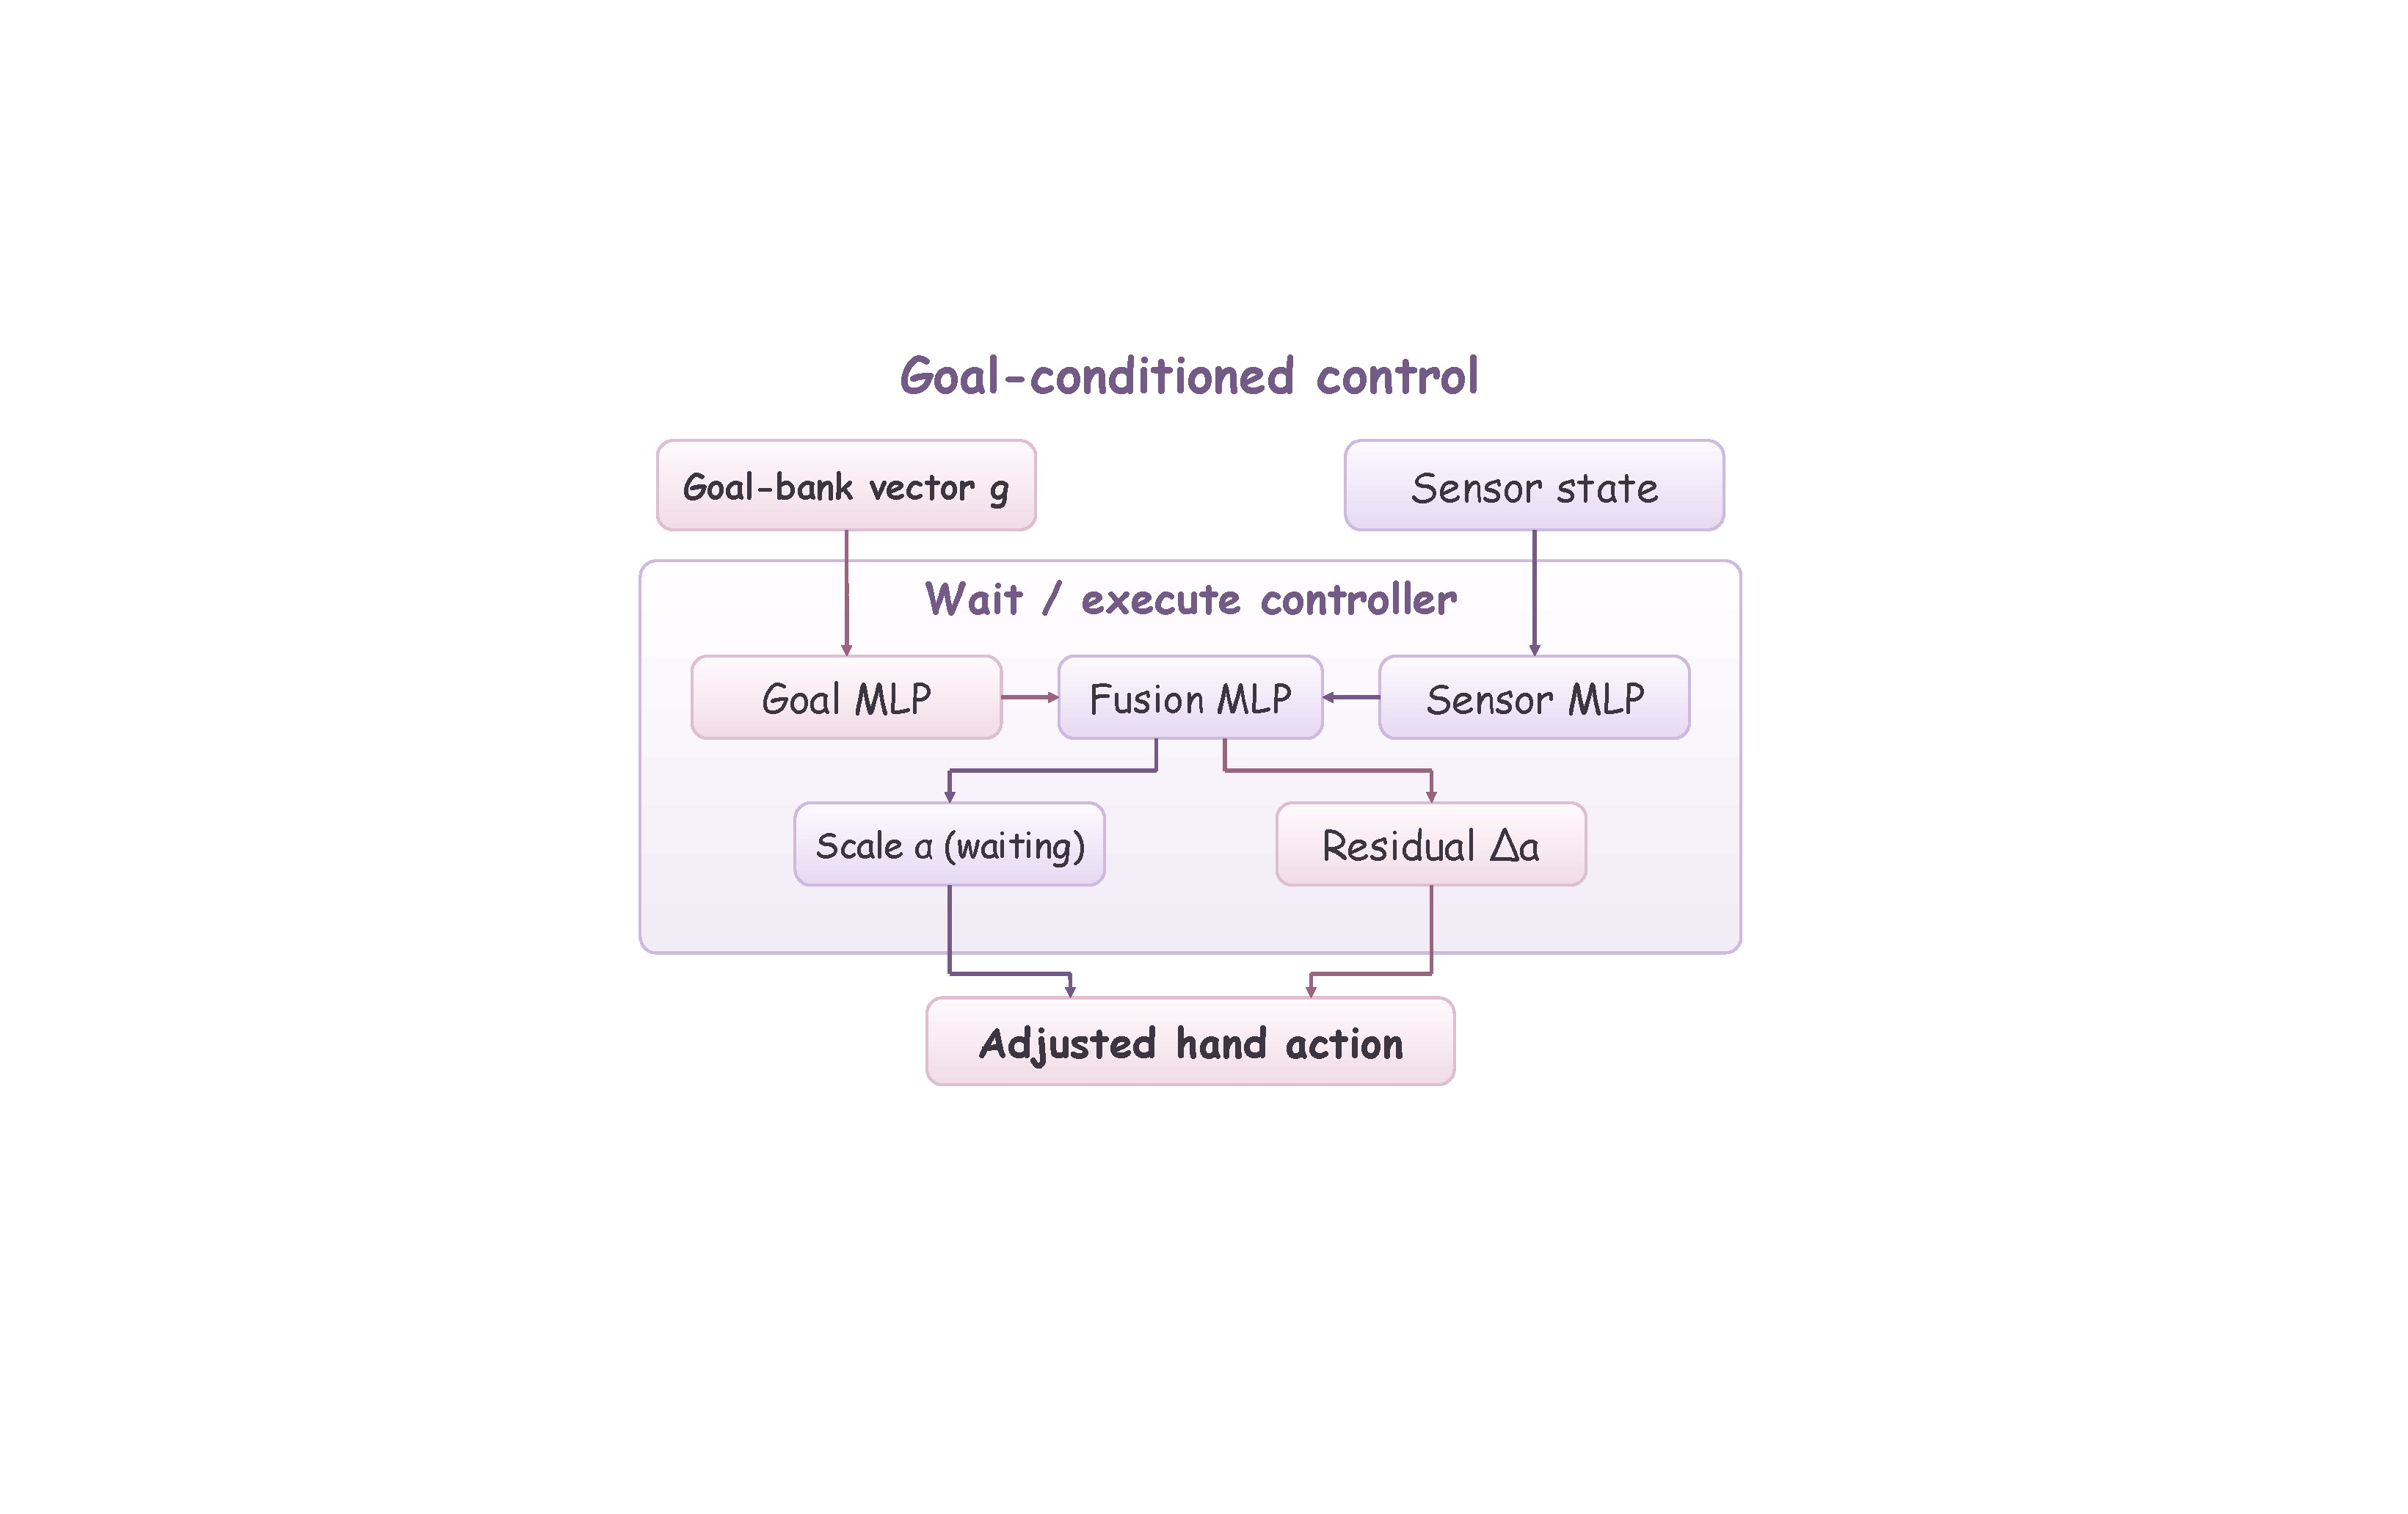
\includegraphics[width=\columnwidth]{figures/imported/reveal_controller_ppt.pdf}
\caption{\textbf{Goal-conditioned local control.} The waiting and execution controllers fuse the goal-bank vector with the sensor state, predict a waiting scale and a bounded joint correction, and produce the adjusted hand action.}
\label{fig:controller-architecture}
\end{figure}

Q1 compares complete systems, which differ in several components. The next two studies change one component at a time, starting with control. What should the hand do while the agent is thinking? Figure~\ref{fig:controller-architecture} summarizes the four controller choices: keep following the student's command, slow it by a fixed coefficient of 0.15, learn the slowing coefficient, or learn slowing together with a bounded joint correction. All four use the same execution controller once a reply has arrived. Each is evaluated on 120 trials, 40 under each of three evaluation seeds, with the trained weights fixed.

Following the student at full speed is the worst choice: 73/120 trials succeed (60.8\%), and 24 end in a drop while waiting. Fixed slowing roughly halves the waiting drops, to 13, and reaches 88/120 (73.3\%). Learning the slowing coefficient alone lowers waiting drops further, to seven, but more trials then fail during execution or for other reasons, so it brings no gain over fixed slowing (82/120, 68.3\%). Adding the joint correction gives the best result on every count: 104/120 successes (86.7\%), five waiting drops and four execution drops. How fast the hand moves is therefore only part of the answer. The controller also needs the freedom to adjust individual joints, and with it gains 13.3 points over fixed slowing. Per-seed results and outcome breakdowns are in the supplement.

A second-object Duck cohort confirms the ordering: the full controller reaches 94/120, versus 67/120 for continued execution and fixed slowing and 73/120 for learned slowing (all Holm-adjusted $p\le1.04\times10^{-4}$). Seed and eligibility details are in the supplement; this is an independent object-specific validation, not a pooled estimate.

\begin{table}[t]
\centering\small
\setlength{\tabcolsep}{2.5pt}
\begin{tabularx}{\linewidth}{@{}Xrrrrr@{}}
\toprule
Waiting policy & Success & \% & \shortstack{Wait\\drops} & \shortstack{Exec.\\drops} & Other\\
\midrule
Continue student & 73/120 & 60.8 & 24 & 14 & 9\\
Fixed slowing & 88/120 & 73.3 & 13 & 8 & 11\\
Learned slowing & 82/120 & 68.3 & 7 & 14 & 17\\
\textbf{Slowing + correction} & \textbf{104/120} & \textbf{86.7} & \textbf{5} & \textbf{4} & \textbf{7}\\
\bottomrule
\end{tabularx}
\caption{\textbf{Q2: controller ablation on the cube.} Outcome counts per method, 120 trials each. Wait and execution drops denote failure stages; Other holds the remaining failures.}
\label{tab:waiting}
\end{table}



\subsection{Q3: Visual Exploration and Feedback}
\begin{figure}[!b]
\centering
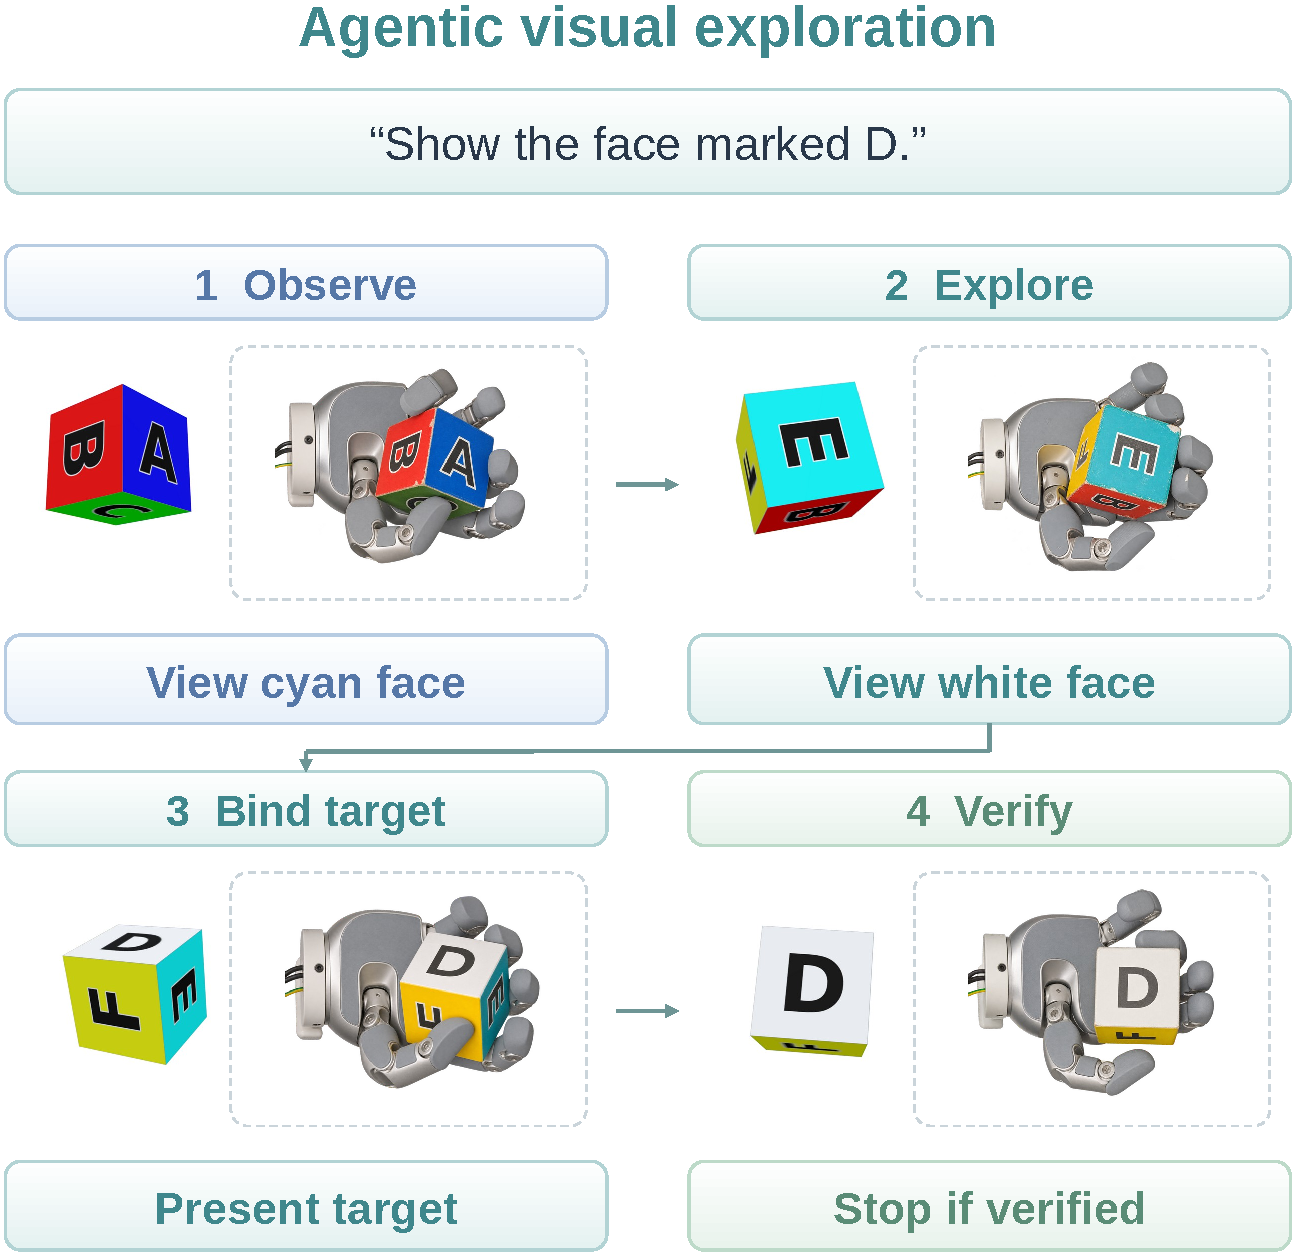
\includegraphics[width=\columnwidth]{figures/imported/v11/reveal_exploration_v11.pdf}
\caption{\textbf{Agentic visual exploration.} Given a request whose face is not in view, the agent observes, chooses an inspection that exposes new faces, binds the target once it appears, and stops only after the requested face is presented. Every step is a decision from the image and the action history, not a fixed schedule.}
\label{fig:exploration}
\end{figure}


We now turn to the agent. Three interventions examine how it acquires and uses evidence (Table~\ref{tab:q3-feedback}): whether it receives feedback at all, whether that feedback contains new images, and whether it chooses its own inspection actions. Each comparison has its own set of 40 matched pairs.

\begin{table}[!htbp]
\centering\small
\begin{tabular}{lrrrr}
\toprule
Condition & Success & \% & Drops & Calls\\
\midrule
\multicolumn{5}{l}{\textbf{(a) Continued feedback: one vs. up to six calls}}\\
\AblationFeedbackRows
\midrule
\multicolumn{5}{l}{\textbf{(b) Fresh visual evidence: same six-call cap}}\\
\ImageRefreshRows
\midrule
\multicolumn{5}{l}{\textbf{(c) Inspection policy: cube}}\\
\InspectionPolicyRows
\midrule
\multicolumn{5}{l}{\textbf{(d) Inspection policy: pig}}\\
\PigInspectionPolicyRows
\bottomrule
\end{tabular}
\caption{\textbf{Q3: visual evidence and inspection choices.} Each comparison uses 40 matched pairs; (a,b) use the cube. In (a), one pair is excluded for a service error, and the feedback arm reuses Q2's first-seed trials. (b) changes only the agent's RGB input. (c,d) change only inspection direction and duration. Drops and calls are totals over all trials.}
\label{tab:q3-feedback}
\label{tab:feedback}
\label{tab:image-refresh}
\end{table}

\paragraph{(a) Does continued feedback help find the target?}
With a single call, the agent sees one image and must plan up to six actions in advance. With continued feedback, it may call up to six times, each with a new image and the action history. Local controllers, stopping and time limits are identical. Success rises from 6/39 to 33/39, and all 27 discordant pairs favor feedback ($p=1.49\times10^{-8}$). The single-call agent usually recognizes that it cannot see the target: it abstains in 28 trials, and feedback turns 22 of these into successes. In 32 feedback trials the first binding comes after an inspection (Fig.~\ref{fig:exploration}).

\paragraph{(b) Does the next image provide useful evidence?}
More calls could help simply by giving the agent more chances. To separate this from visual evidence, both conditions here have the same six-call cap, live numeric feedback, history and local control, and differ only in the image: the current view, or the first frame repeated at every call. Success is 32/40 with current images and 9/40 with the repeated frame; all 23 discordant pairs favor current images ($p=2.38\times10^{-7}$). The nine repeated-frame successes are exactly the trials in which both arms bind correctly on the first call, before any new view is needed. Beyond these, current images produce 25 further correct bindings, 23 of which end in success, and the repeated frame produces none. The gain comes from what the new images show.

\paragraph{(c) Does choosing inspection actions help?}
We next fix the evidence channel and vary who chooses the inspection. In the adaptive arm the agent selects the direction and duration of each inspection. In the fixed arm, inspections follow a prescribed sweep over the six skills, three seconds each; the agent still decides when to inspect, bind or abstain. Model, controllers, image input, history format and stopping are shared.

On the pig, adaptive inspection succeeds in 37/40 trials (92.5\%) against 29/40 (72.5\%) for the fixed sweep. Eight pairs favor adaptive inspection and none favor the sweep ($p=0.0078$). The difference lies in finding the target: correct terminal bindings number 37 versus 29, while each arm drops the object twice. Adaptive inspection also needs 15.2\% fewer calls and 26.1\% fewer tokens. On the cube, the rates are 38/40 (95.0\%) versus 31/40 (77.5\%), with nine pairs favoring adaptive inspection and two favoring the sweep. The effect has the same direction and a similar size, but does not reach significance with 40 pairs ($p=0.065$). The pig comparison and its analysis were fixed before its trials were run. The supplement reports seed splits, binding trajectories and costs for both objects.

\subsection{Q4: Pose Estimation and Sim-to-Real Transfer}
\begin{figure}[!t]
\centering
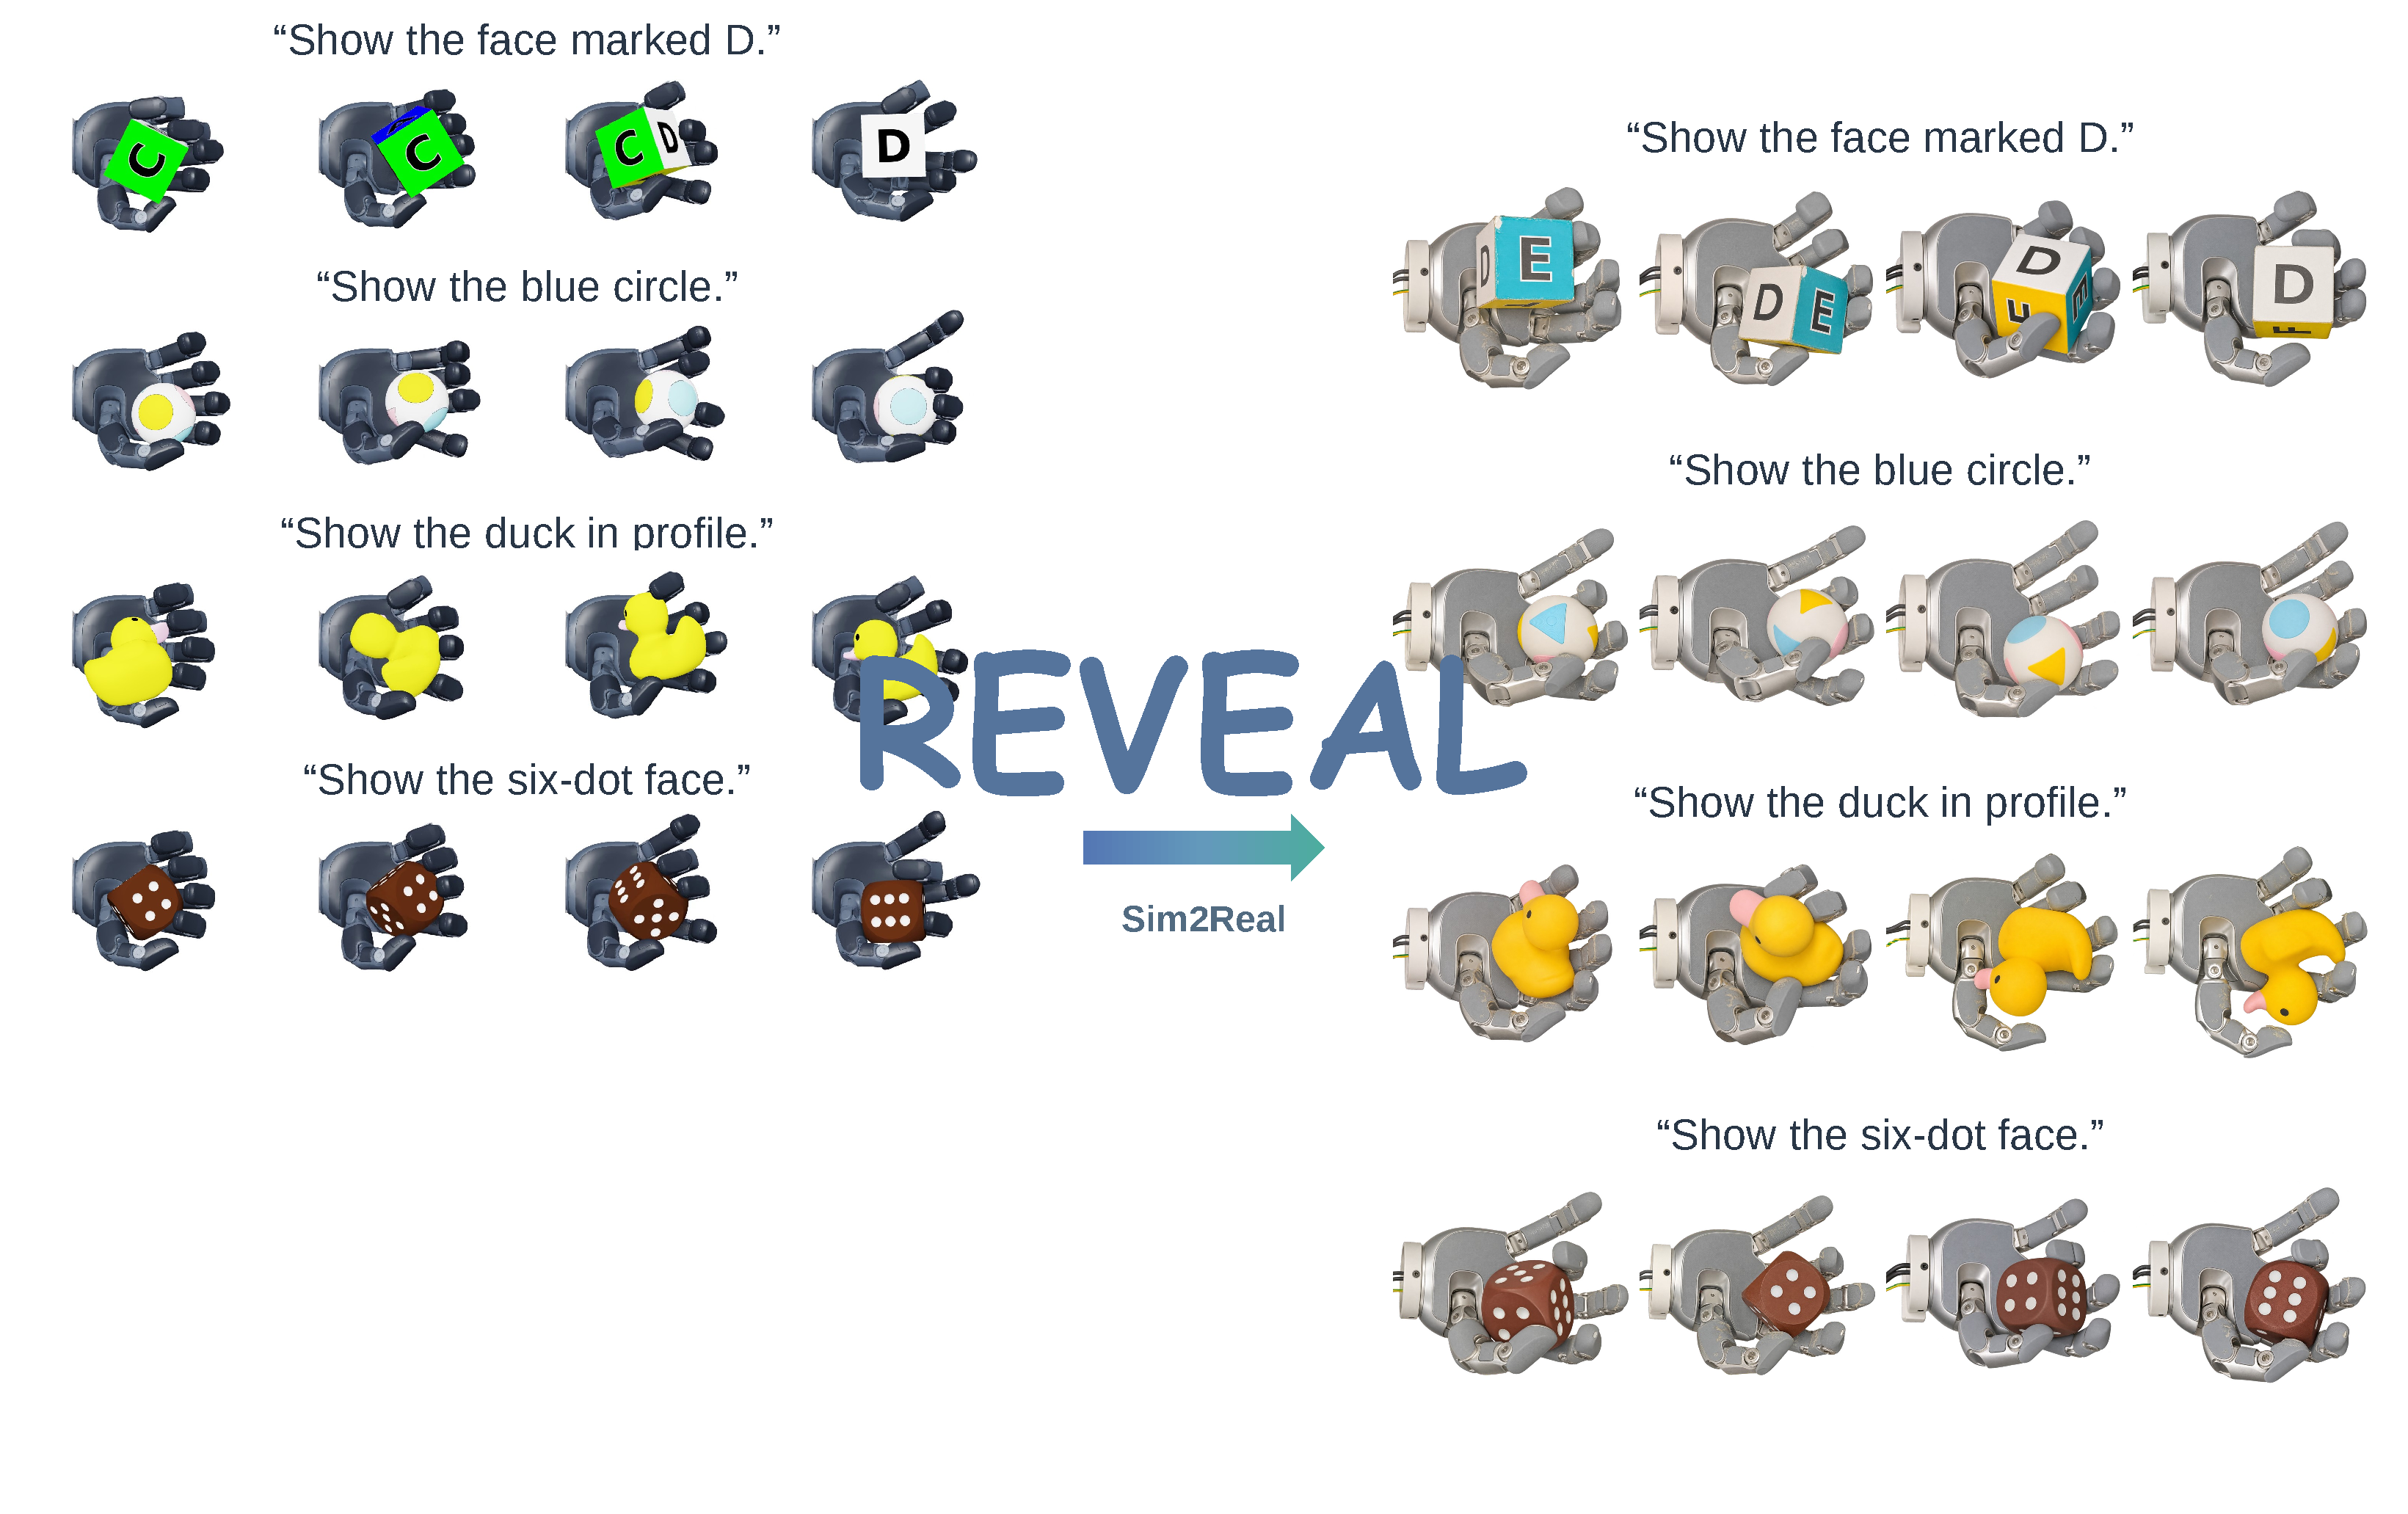
\includegraphics[width=\columnwidth]{figures/imported/reveal_sim_real_ppt.pdf}
\caption{\textbf{Evaluation objects and physical transfer.} The same target-presentation task is evaluated across six simulated objects and four objects on the physical hand.}
\label{fig:sim-real-overview}
\end{figure}

\paragraph{Pose estimation under hand occlusion.}
We compare our estimator with a ViserDex-style baseline that regresses the same keypoints from the image alone and is trained for the same object and camera~\cite{bhardwaj2026viserdex} (Table~\ref{tab:pose-summary}). In simulation we use 6,144 frames rendered with real-camera calibration, Gaussian-splat appearance and hand occlusion. Over all frames, 10\,mm/$10^\circ$ recall rises from 37.5\% to 64.7\%, and invalid predictions fall from 69 to one. The average hides a strong dependence on occlusion, because the test set deliberately includes camera pitches up to $105^\circ$, at which much of the object is hidden. When less than a quarter of the object is hidden, our estimator is correct in 97.6\% of frames against 66.2\% for the baseline, and at the nominal camera view it reaches 99.8\%. Between 25\% and 50\% occlusion its recall is 55.5\% (baseline: 19.9\%); beyond that both fail.

The gap carries over to real images. On 1,000 frames of the cube being rotated in the hand, scored against a multi-view FoundationPose reference~\cite{wen2024foundationpose}, our estimator reaches 87.3\% recall and the baseline 40.7\% (protocol in the supplement). We use our estimator in all simulated and physical experiments.

\begin{table}[!htbp]
\centering\small
\setlength{\tabcolsep}{4pt}
\begin{tabular}{lrrr}
\toprule
 & \multicolumn{2}{c}{Simulation} & Real\\
\cmidrule(lr){2-3}\cmidrule(lr){4-4}
Estimator & 10\,mm / 10$^\circ$ & 5\,mm / 5$^\circ$ & 10\,mm / 10$^\circ$\\
\midrule
ViserDex-style & 37.53 & 14.63 & 40.7\\
\textbf{Ours} & \textbf{64.73} & \textbf{47.56} & \textbf{87.3}\\
\bottomrule
\end{tabular}
\caption{\textbf{Q4: pose recall (\%) on the cube under hand occlusion.} Recall requires both errors below the listed thresholds.}
\label{tab:pose-summary}
\end{table}


\paragraph{Real-hand evaluation.}
We run Rule, Fine-tuned and REVEAL on a physical Revo3 hand with four of the simulated objects (cube, die, ball and duck), 20 trials per object and method (240 in total). A RealSense D405 camera provides the images for pose estimation. A trial succeeds when the hand presents the requested target within $15^\circ$ of its reference orientation and stops without dropping the object. REVEAL completes 70/80 trials (\HardwareAimiSuccess\%), against \HardwareFineTunedSuccess\% for Fine-tuned and \HardwareRuleSuccess\% for Rule, a margin of \HardwareGain{} points over the stronger baseline (Table~\ref{tab:hardware-results}). The ranking of the three methods is the same for every object, and the duck is the hardest object for all of them. Object descriptions, targets and the scoring setup are given in the supplement.

\begin{table}[!htbp]
\centering\small
\setlength{\tabcolsep}{2.5pt}
\resizebox{\columnwidth}{!}{%
\begin{tabular}{lcccc}
\toprule
\multirow{2}{*}{Object} & \multirow{2}{*}{Rule} & \multirow{2}{*}{Fine-tuned} & Fine-tuned & \multirow{2}{*}{REVEAL}\\
 & & & + ctrl. & \\
\midrule
Cube & 9/20 (45\%) & 15/20 (75\%) & 14/20 (70\%) & \textbf{18/20 (90\%)}\\
Die & 8/20 (40\%) & 14/20 (70\%) & 14/20 (70\%) & \textbf{18/20 (90\%)}\\
Ball & 9/20 (45\%) & 13/20 (65\%) & 12/20 (60\%) & \textbf{19/20 (95\%)}\\
Duck & 6/20 (30\%) & 11/20 (55\%) & 10/20 (50\%) & \textbf{15/20 (75\%)}\\
\midrule
Total & 32/80 (40\%) & 53/80 (66.25\%) & 50/80 (62.5\%) & \textbf{70/80 (87.5\%)}\\
\bottomrule
\end{tabular}}
\caption{\textbf{Q4: real-hand task completion.} Successes/trials, 20 per object and method.}
\label{tab:hardware-results}
\end{table}


% Continue directly into discussion so the main paper stays within the eight-page body limit.
\section{Discussion}

A language target has to be made visible before it can be made a goal, and in a hand the act of making it visible is the act that puts the grasp at risk. REVEAL handles this by separating the rate at which the object is understood from the rate at which it is held. The controlled studies support each part, but the more useful reading is that the parts are not independent: fresh images only help an agent that also chooses what to look at, and only an agent that chooses what to look at produces the long occlusions that make the local controllers necessary. The changed-mapping study says the same thing from the other side, since a system that learned the mapping collapses when the mapping moves while one that explores does not.

\paragraph{Limitations.}
The evaluation covers one hand, one camera and six objects whose marks are legible letters and dot counts; transparent, reflective and deformable objects are untested. Every experiment uses a hosted vision-language model under a fixed call cap, so the reported latencies belong to that service and a slower or weaker model might not close the loop at all. Quantitative claims come from simulation, and the physical study covers four objects with 20 trials per cell, so the hardware margins indicate a consistent direction rather than a calibrated effect size. We also assume the object stays in the hand: both pose estimators fail beyond roughly half occlusion, and recovery after a drop is outside the scope of the method.

\clearpage
\section*{LLM Usage Statement}
OpenAI Codex assisted with research discussion, implementation, experiment orchestration, literature retrieval, statistical analysis, figure-layout code, and drafting and editing throughout the manuscript. A hosted vision-language model and Qwen3-VL are evaluated system components. Numerical claims are grounded in recorded experiments. Unfinished work is identified explicitly. The authors are responsible for verifying the text, references, code, figures, and results before submission.
{\small\bibliographystyle{ieeenat_fullname}\bibliography{references}}
\end{document}
